\documentclass[conference]{IEEEtran}
\IEEEoverridecommandlockouts

\usepackage{fontspec}
\usepackage{polyglossia}
\setmainlanguage{russian}
\setotherlanguage{english}
\setmainfont{Times New Roman}

\usepackage{cite}
\usepackage{amsmath,amssymb,amsfonts}
\usepackage{algorithmic}
\usepackage{graphicx}
\usepackage{float}
\usepackage{textcomp}
\usepackage{xcolor}
\usepackage{booktabs}
\usepackage{array}
\usepackage{tabularx}
\usepackage{multirow}
\usepackage{hyperref}
\usepackage{microtype}
\usepackage{caption}

\def\BibTeX{{\rm B\kern-.05em{\sc i\kern-.025em b}\kern-.08em
    T\kern-.1667em\lower.7ex\hbox{E}\kern-.125emX}}

\begin{document}

\title{Beyond Gaussian Noise: Convergence of Stochastic Optimizers under Correlated and Heavy-Tailed Financial Gradient Noise}

\author{%
\IEEEauthorblockN{Дмитрий\,Кортунов}
\IEEEauthorblockA{\textit{НИУ ВШЭ}\\
Москва, Россия\\
dvkortunov@edu.hse.ru}
\and
\IEEEauthorblockN{Вадим\,Пастушенко}
\IEEEauthorblockA{\textit{НИУ ВШЭ}\\
Москва, Россия\\
vapastushenko@edu.hse.ru}
\and
\IEEEauthorblockN{Алексей\,Дубовицкий}
\IEEEauthorblockA{\textit{НИУ ВШЭ}\\
Москва, Россия\\
andubovitskiy@edu.hse.ru}
\and
\IEEEauthorblockN{Андрей\,Шадрин}
\IEEEauthorblockA{\textit{НИУ ВШЭ}\\
Москва, Россия\\
arshadrin@edu.hse.ru}
}

\maketitle

\begin{abstract}
Финансовые временные ряды содержат шум различной природы: гауссов,
тяжёлохвостовый, коррелированный и их комбинации. Прямая подача таких
данных в стандартные стохастические оптимизаторы нарушает базовые
предположения теории сходимости. Мы исследуем альтернативный подход:
перед оптимизацией применяется этап шумоподавления~--- скользящее среднее,
фильтр Калмана, вейвлет-пороговая обработка или медианная фильтрация,~---
после чего ряд подаётся в SGD, Adam или AdamW. Основной вопрос: насколько
выбор фильтра влияет на скорость сходимости и итоговое качество модели,
и можно ли подобрать пару (фильтр, оптимизатор), устойчивую к нескольким
типам шума одновременно? Мы формализуем задачу как факторный эксперимент
(тип~шума)~$\times$~(фильтр)~$\times$~(оптимизатор), формулируем явные
гипотезы из теоретических свойств методов и проверяем их на синтетических
и реальных финансовых рядах. Ключевой результат: при $\alpha$-устойчивом
шуме причинная медиана переводит расходящийся SGD в сходящийся режим и снижает
асимптотический уровень $\|\nabla f\|^2$ на один-два порядка, тогда как линейные
фильтры эффекта не дают; результат сохраняется при индексе хвоста, измеренном на
реальных рядах. При гауссовом шуме фильтрация нейтральна или слегка вредит.
Важная оговорка: на реальных данных фильтр ускоряет и стабилизирует
\emph{оптимизацию}, но \emph{прогноз} на отложенной выборке не улучшает.
\end{abstract}

\begin{IEEEkeywords}
шумоподавление, финансовые временные ряды, стохастическая оптимизация,
фильтр Калмана, вейвлет-порог, медианная фильтрация, Adam, SGD, сходимость
\end{IEEEkeywords}


%--------------------------------------------------------------------
\section{Введение}
%--------------------------------------------------------------------

В обучении на финансовых временных рядах стандартно фокусируются либо на
выборе архитектуры модели, либо на модификациях оптимизатора. При этом сама
структура входного шума часто остаётся «за кадром», хотя для финансовых
данных именно она задаёт сложность обучения: тяжёлые хвосты, долгая память
и выбросы нарушают предпосылки, при которых гарантируется стабильная работа
классических стохастических методов.

В работе мы рассматриваем шумоподавление не как вспомогательную технику
визуализации, а как полноценную часть оптимизационного процесса. Гипотеза
состоит в том, что правильная предобработка может существенно изменить
свойства градиентного шума и тем самым ускорить сходимость без усложнения
самого оптимизатора.

Эмпирически мы сравниваем матрицу
(тип~шума)~$\times$~(фильтр)~$\times$~(оптимизатор) на синтетических и
реальных финансовых данных и отвечаем на практический вопрос: когда
предобработка действительно помогает, а когда её эффект минимален или даже
вреден из-за пересглаживания полезного сигнала. Короткий ответ, который мы
получаем уже на первых экспериментах: при тяжёлых хвостах предобработка
меняет сходимость, и сильно; при гауссовом шуме~--- нет.

\textbf{Структура работы.} Раздел~\ref{sec:related} помещает работу в
контекст литературы. Раздел~\ref{sec:setup} вводит модель ряда, классы
шума, задачу прогноза и формализует исследовательскую задачу как факторный
эксперимент с измеримыми метриками. Раздел~\ref{sec:background} даёт
теоретический фон по фильтрам и оптимизаторам, формулирует предпосылки и
явные гипотезы. Разделы~\ref{sec:exp1}--\ref{sec:exp3} описывают три
эксперимента (синтетика, калибровка под реальные данные, реальные ряды) и
проверяют гипотезы. Раздел~\ref{sec:practice} выводит практические критерии
выбора пары (фильтр, оптимизатор) и явно указывает основание каждого из них.
Раздел~\ref{sec:problems} обсуждает ограничения, включая нерешённый случай
смешанного шума.

\section{Обзор литературы}
\label{sec:related}

\subsection{Фильтрация временных рядов}

Фильтр Калмана~\cite{kalman1960} для финансовых приложений подробно
разобран у Harvey~\cite{harvey1990kalmanfinance}. Теория вейвлет-порогового
шумоподавления восходит к работе Donoho и Johnstone~\cite{donoho1994wavelets};
базисы Добеши~\cite{daubechies1992wavelets} стали стандартом практики.
Медианную фильтрацию и её взвешенные обобщения систематически изложили
Yin~et~al.~\cite{yin1996median}.

\subsection{Природа финансового шума}

Cont~\cite{cont2001} зафиксировал набор устойчивых эмпирических фактов
для доходностей: тяжёлые хвосты, кластеризация волатильности, медленное
убывание автокорреляций абсолютных значений. Мандельброт~\cite{mandelbrot1963}
предложил $\alpha$-устойчивые распределения в качестве модели ещё в
1963~году. \c{S}im\c{s}ekli~et~al.~\cite{simsekli2019tailindex} показали,
что стохастический градиент при обучении нейросетей демонстрирует те же
признаки~--- $\alpha$-устойчивость с $\alpha$ заметно меньше двух.

\subsection{Стохастическая аппроксимация при нестандартном шуме}

Asymptotic-уровень: Anantharam и Borkar~\cite{anantharam2012sa} исследуют
стохастическую аппроксимацию при одновременно тяжёлом и долгозависимом
шуме методом предельного ОДУ. Первые
конечновременные гарантии при обоих эффектах сразу получены в недавней
работе Chandak~et~al.~\cite{chandak2026hl}. Направление робастной
оптимизации через обрезание градиентов развито у Gorbunov~et~al.~\cite{gorbunov2020clipping}
и Zhang~et~al.~\cite{zhang2020clipping}; вероятностные гарантии для
невыпуклого случая~--- у Cutkosky и Mehta~\cite{cutkosky2021high}.

\subsection{Место данной работы}

Перечисленные работы либо анализируют поведение конкретного оптимизатора
при заданном типе шума, либо изучают свойства фильтров как таковых.
Совместное влияние выбора фильтра и оптимизатора при тяжёлохвостовом и
коррелированном финансовом шуме эмпирически не измерялось. Открытого
бенчмарка формата (фильтр\,$\times$\,шум\,$\times$\,оптимизатор) на
финансовых рядах нам обнаружить не удалось.

%--------------------------------------------------------------------
\section{Модель ряда и постановка задачи}
\label{sec:setup}
%--------------------------------------------------------------------

В этом разделе мы вводим только то, что нужно для постановки
исследовательской задачи: модель наблюдаемого ряда, классы шума, задачу
прогноза и формальное описание изучаемого пространства экспериментов.
Конкретные фильтры и оптимизаторы как алгоритмы описаны отдельно, в
разделе~\ref{sec:background}.

\subsection{Наблюдательная модель и классы шума}

Наблюдаемый ряд $y_1,\dots,y_T\in\mathbb{R}$ описывается стандартной
аддитивной моделью
\begin{equation}
  y_t = s_t + \xi_t,
  \label{eq:model}
\end{equation}
где $s_t$~--- полезный сигнал, $\xi_t$~--- шум. Цель предобработки~---
оценить $s_t$ по доступным к моменту $t$ наблюдениям, не используя
будущее. Мы рассматриваем четыре класса шума, охватывающих основные
режимы, встречающиеся в финансовых данных.

\textbf{N1~--- гауссов белый}, $\xi_t\sim\mathcal{N}(0,\sigma^2)$. Это
контрольный случай, при котором теория сходимости SGD работает в полную
силу.

\textbf{N2~--- розовый ($1/f$)}: $\xi_t = \sum_{j\ge0}\psi_j\eta_{t-j}$ с
гауссовыми инновациями $\eta_j$ и коэффициентами FARIMA$(0,d,0)$,
$d\in(0,1/2)$. Дисперсия конечна, но корреляции убывают медленно (долгая
память).

\textbf{N3~--- тяжёлохвостовый}, $\xi_t\sim S_\alpha(\sigma,0,0)$,
$\alpha\in(1,2)$. Моменты порядка $p\ge\alpha$ бесконечны. Именно этот
режим наиболее близок к реальным финансовым данным.

\textbf{N4~--- смешанный}: $\alpha$-устойчивые инновации, пропущенные через
$1/f$-фильтр. Тяжёлые хвосты и долгая память присутствуют одновременно.

\subsection{Задача прогноза ряда}
\label{sec:forecast}

Центральная прикладная задача~--- краткосрочный одношаговый прогноз.
Используем причинную AR($p$)-модель. На шаге $t>p$ входом служит вектор
последних $p$ наблюдений
\begin{equation}
  \phi_t = [\tilde y_{t-1}, \tilde y_{t-2}, \dots, \tilde y_{t-p}]^\top
  \in \mathbb{R}^{p},
  \label{eq:ar_input}
\end{equation}
где $\tilde y$~--- либо исходный ряд $y$, либо его версия, обработанная
причинным фильтром. Выход модели~--- одношаговый прогноз
\begin{equation}
  \hat y_t = x^\top \phi_t,
  \label{eq:ar_output}
\end{equation}
$x\in\mathbb{R}^{p}$~--- вектор авторегрессионных коэффициентов. При
обучении модель восстанавливает следующее значение того же ряда
$\tilde y$, по которому построены признаки: каждый объект~--- пара
$(\phi_t, \tilde y_t)$, а минимизируемая функция потерь квадратична:
\begin{equation}
  f(x)=\frac{1}{n}\sum_{t=p+1}^{p+n}\bigl(x^\top \phi_t - \tilde y_t\bigr)^2.
  \label{eq:ar_loss}
\end{equation}
Таким образом, фильтрация влияет и на входные признаки $\phi_t$, и (при
$F\neq F_0$) на обучающий таргет $\tilde y_t$. \emph{Качество} же
оценивается отдельно, на отложенной части ряда, по \emph{исходному}
будущему значению $y_t$: прогноз $x^\top\phi_t$ сравнивается с $y_t$, а не
с его сглаженной версией. Именно сравнение с исходным рядом на holdout
исключает ситуацию, в которой фильтр оценивался бы по им же сглаженному
таргету.

\subsection{Вспомогательные целевые функции}
\label{sec:aux}

Чтобы изолированно измерить влияние шума на сходимость, не путая его с
особенностями конкретной прогнозной модели, мы дополнительно используем
две «чистые» задачи оптимизации, в которые шум ряда попадает прямо в
признаки и тем самым в градиент. Они служат \emph{диагностическим
инструментом}, а не самостоятельной целью.

\emph{Квадратичная} (при положительно определённой $A\in\mathbb{R}^{d\times d}$
и $b\in\mathbb{R}^d$):
\begin{equation}
  f(x) = \tfrac{1}{2}x^\top A x - b^\top x,
  \label{eq:quadratic}
\end{equation}
с единственным минимумом $x^* = A^{-1}b$. Гладкий выпуклый ландшафт без
нелинейностей позволяет приписать любое замедление сходимости именно
шуму, а не геометрии потерь.

\emph{Логистическая регрессия} (при наборе $\{(\phi_t,c_t)\}_{t=1}^n$,
$\phi_t\in\mathbb{R}^d$~--- лаговые признаки из ряда $y$,
$c_t\in\{0,1\}$~--- метка):
\begin{equation}
  f(x) = -\frac{1}{n}\sum_{t=1}^{n}
    \bigl[c_t\log\sigma(x^\top\phi_t)
         +(1-c_t)\log(1-\sigma(x^\top\phi_t))\bigr].
  \label{eq:logreg}
\end{equation}
Она добавляет к диагностике невырожденную, но по-прежнему выпуклую
нелинейность.

Все три задачи~--- AR-прогноз~\eqref{eq:ar_loss}, квадратичная и
логистическая~--- объединены тем, что шум ряда $y$ входит в них через
признаки и, значит, через стохастический градиент.

\subsection{Формализация исследовательской задачи}
\label{sec:research}

Перед оптимизацией весь ряд проходит через фильтр $F$:
$\tilde{y} = F(y_1,\dots,y_T)$ (причём только причинно). Признаки строятся
из $\tilde{y}$, а мини-батчевый градиент на итерации $k$ равен
\begin{equation}
  g_k = \frac{1}{|\mathcal{B}_k|}\sum_{t\in\mathcal{B}_k}
        \nabla_x\ell(x_k,\tilde{\phi}_t,c_t).
  \label{eq:grad}
\end{equation}
Параметры обновляются как $x_{k+1}=x_k-\eta\,\phi(g_k)$, где $\phi(\cdot)$
задаёт конкретный оптимизатор.

\textbf{Изучаемое пространство.} Исследовательская задача~--- измерить, как
тройка
\[
  (\text{тип шума }\mathcal{N})\times(\text{фильтр }F)\times(\text{оптимизатор }A)
\]
влияет на сходимость и качество. Все три оси перебираются полным
факторным дизайном (раздел~\ref{sec:exp1}).

\textbf{Метрики.} Основная метрика~--- медианное (по~100~запускам) число
итераций до $\varepsilon$-точности:
\begin{equation}
  T(\varepsilon;F,A,\mathcal{N})
  = \min\{K:\mathbb{E}\|\nabla f(x_K)\|^2\le\varepsilon\}.
  \label{eq:metric}
\end{equation}
Дополнительно измеряем \emph{бинарную сходимость}~--- долю запусков,
достигших 100-кратного снижения $\|\nabla f\|^2$,~--- и
\emph{асимптотический уровень} $\|\nabla f\|^2$~--- медиану финального
$\|\nabla f\|^2$ по последним 200~итерациям (в таблицах сокращаем до
«асимпт.»). Бинарная сходимость отвечает на вопрос «сходится ли вообще»,
а асимптотический уровень~--- «насколько глубоко».

Важно, что три метрики дополняют друг друга и применимы в разных
режимах. При $\alpha$-устойчивом шуме итерация может вообще не иметь
конечного предела (раздел~\ref{sec:premises}); тогда $T(\varepsilon)$ не
определено (формально равно горизонту), и информативны именно бинарная
сходимость и асимптотический уровень. Поэтому для режима тяжёлых хвостов
(H1) мы считаем первичными бинарную сходимость и этот уровень,
а $T(\varepsilon)$
приводим там, где сходимость достигается; для уже сходящихся адаптивных
методов (H2) первична скорость $T(\varepsilon)$.

%--------------------------------------------------------------------
\section{Теоретический фон, предпосылки и гипотезы}
\label{sec:background}
%--------------------------------------------------------------------

Здесь мы описываем сравниваемые методы как алгоритмы, кратко напоминаем их
теоретические свойства и из этих свойств выводим явные гипотезы, которые
затем проверяются экспериментально.

\subsection{Фильтры}
\label{sec:filters}

Рассматриваем шесть режимов предобработки; все причинные (при вычислении
$\tilde{y}_t$ используются только $y_1,\dots,y_t$).

\begin{itemize}
  \item \textbf{F0~--- без фильтрации} ($\tilde{y}_t = y_t$), контроль.
  \item \textbf{F1~--- скользящее среднее} по $w$ последним наблюдениям.
        Линейный сглаживатель; оптимален в среднеквадратичном смысле для
        стационарного гауссова шума без памяти.
  \item \textbf{F2~--- фильтр Калмана} с моделью случайного блуждания
        $s_t = s_{t-1}+w_t$; оптимальная линейная оценка при гауссовом
        шуме~\cite{kalman1960}.
  \item \textbf{F3~--- вейвлет-пороговая обработка} в базисе
        Добеши~\cite{donoho1994wavelets,daubechies1992wavelets}.
        Разреженно представляет кусочно-регулярный сигнал и эффективно
        подавляет коррелированный ($1/f$) шум за счёт пороговой обрезки
        мелкомасштабных коэффициентов.
  \item \textbf{F4~--- причинная медиана} по $w$ последним наблюдениям.
        Единственный из простых фильтров, устойчивый к
        выбросам~\cite{yin1996median}: одиночный экстремальный отсчёт не
        сдвигает медиану окна.
  \item \textbf{F5~--- каскад F4$\to$F3}: причинная медиана против
        $\alpha$-устойчивых выбросов, затем вейвлет против остаточной
        $1/f$-памяти. Двухстадийная попытка закрыть смешанный режим N4;
        разбор в §\ref{sec:cascade}.
\end{itemize}

\subsection{Оптимизаторы}
\label{sec:opt}

Обновление имеет общий вид $x_{k+1}=x_k-\eta\,\phi(g_k)$:
\begin{itemize}
  \item \textbf{SGD}: $\phi(g)=g$~--- базовый случай.
  \item \textbf{Clipped-SGD}: $\phi(g)=\min(1,\tau/\|g\|)\,g$~---
        обрезание ограничивает вклад редких больших градиентов.
  \item \textbf{Normalized-SGD}: $\phi(g)=g/\|g\|$~--- полное удаление
        масштаба градиента.
  \item \textbf{Adam}~\cite{kingma2015adam} и
        \textbf{AdamW}~\cite{loshchilov2019adamw}~--- адаптивные методы с
        покоординатным масштабированием по вторым моментам.
\end{itemize}

\subsection{Предпосылки}
\label{sec:premises}

Классический анализ SGD предполагает конечную дисперсию градиентного
шума. При $\alpha$-устойчивом шуме с $\alpha<2$ это предположение
нарушается: второй момент бесконечен, и редкие гигантские шаги не дают
итерации стабилизироваться у минимума~\cite{simsekli2019tailindex,
gorbunov2020clipping}. Отсюда две принципиально разные стратегии борьбы:
(i)~подавить выбросы \emph{на входе} робастным фильтром (F4), вернув
градиентному шуму конечную дисперсию; (ii)~ограничить выбросы \emph{внутри}
оптимизатора (обрезание, нормировка, адаптивные моменты). Долгая память
($1/f$) дисперсию не ломает, но коррелирует последовательные градиенты;
здесь помогает спектральное разреживание (вейвлет, F3) или адаптивное
усреднение (Adam).

\paragraph{Почему медиана возвращает конечную дисперсию.}
Зафиксируем, отчего робастный фильтр в принципе обязан помочь при
$\alpha<2$. Пусть в окне фильтра наблюдения суть
$y_i=s+\xi_i$, где $\xi_i$~--- н.о.р.\ симметричный $\alpha$-устойчивый
шум, $0<\alpha<2$, так что $\mathbb{E}|\xi_i|^2=\infty$. Для среднего
$\bar y$ это фатально: $\mathrm{Var}(\bar y)=\infty$, и градиентный шум
наследует бесконечный второй момент. Для выборочной медианы $m=\mathrm{med}(y_i)$
по окну размера $w$ ситуация иная.

\emph{Утверждение.} Порядок хвоста выборочной медианы зависит и от
$\alpha$, и от размера окна~--- $\alpha$ никуда не девается. Медиана окна
из $w$ точек превышает уровень $t$ только тогда, когда $t$ превышают не
менее $\lceil w/2\rceil$ из них; так как $\Pr(|\xi|>t)\sim C\,t^{-\alpha}$,
\[
  \Pr(|m-s|>t)\;\sim\;\binom{w}{\lceil w/2\rceil}\,
  \bigl(C\,t^{-\alpha}\bigr)^{\lceil w/2\rceil}
  \;=\;\Theta\!\bigl(t^{-\alpha\lceil w/2\rceil}\bigr).
\]
То есть хвост медианы имеет порядок $\alpha\lceil w/2\rceil$, и конечны её
моменты всех порядков $r<\alpha\lceil w/2\rceil$. Конечная дисперсия
($r=2$) требует $\alpha\lceil w/2\rceil>2$. Для минимального нечётного окна
$w=3$ (хвост $\sim t^{-2\alpha}$) это значит $\alpha>1$; для окна $w=9$,
которое мы используем ($\lceil w/2\rceil=5$), достаточно $\alpha>0.4$~---
с большим запасом при измеренном $\alpha\approx1.2$. $\square$

Конечный второй момент медианы снимает ровно тот барьер, который ставит
$\alpha$-устойчивый шум,~--- бесконечную дисперсию. Это одна из предпосылок
теории Роббинса--Монро, и сама по себе она сходимость не гарантирует
(нужны ещё условия на шаги $\sum_k\gamma_k=\infty$, $\sum_k\gamma_k^2<\infty$,
несмещённость и достаточная регулярность градиента); но без конечной
дисперсии классические гарантии неприменимы вовсе. Линейные фильтры
(F1~MA, F2~Калман) этого барьера не снимают: они \emph{линейны} по входу,
поэтому $\mathrm{Var}(\text{выход})\propto\mathrm{Var}(\xi)=\infty$~--- любая
выпуклая комбинация $\alpha$-устойчивых остаётся $\alpha$-устойчивой.
Отсюда асимметрия, которую мы и наблюдаем эмпирически: при N3 пол
снижает только нелинейная медиана F4, а F1--F3~--- нет
(табл.~\ref{tab:rescue}). Статистический критерий из
раздела~\ref{sec:stats} измеряет ровно эту разницу дисперсий, и потому
эффект выходит столь крупным ($d\approx4$--$11$): мы сравниваем конечную
дисперсию с бесконечной.

\subsection{Гипотезы}
\label{sec:hyp}

Из этих предпосылок мы формулируем четыре проверяемые гипотезы, по одной
на каждый режим шума:

\begin{itemize}
  \item \textbf{H1 (тяжёлые хвосты, N3).} Причинная медиана F4 переводит
        SGD из расходящегося режима в сходящийся и заметно снижает
        асимптотический уровень $\|\nabla f\|^2$; линейные фильтры
        (F1, F2, F3) этого не делают, так как не устойчивы к выбросам.
  \item \textbf{H2 (долгая память, N2).} Для адаптивных методов (Adam,
        AdamW) вейвлет-фильтр F3 ускоряет сходимость сильнее линейных
        сглаживателей.
  \item \textbf{H3 (смешанный шум, N4).} Ни один \emph{простой}
        (одностадийный) фильтр не снижает асимптотический уровень: медиана видит
        одиночный выброс, но долгая память «растягивает» его в кластер,
        не помещающийся в окно.
  \item \textbf{H4 (гауссов контроль, N1).} Фильтрация в лучшем случае
        нейтральна, а медиана слегка проигрывает среднему, для которого
        гауссов шум оптимален.
\end{itemize}

\section{Эксперимент 1: синтетика}
\label{sec:exp1}

\subsection{Дизайн}

Полный факторный эксперимент над тремя задачами (квадратичная регрессия
$d=20$, логистическая классификация $d=15$, авторегрессия AR(5)), всеми
четырьмя типами шума (N1, N2, N3 с $\alpha=1.2$, N4) и шестью фильтрами
(F0--F4 плюс каскад F5~--- двухстадийная причинная предобработка
F4$\to$F3, см.\ §\ref{sec:cascade}). По~100~независимых запусков на каждую
ячейку; гиперпараметры
одинаковы для всех ячеек~--- никакого подбора под конкретный фильтр.

Оптимизаторы естественно делятся на две группы, поэтому факторный
дизайн организован в два связанных блока (это разделение отвечает разным
гипотезам):
\begin{itemize}
  \item \textbf{Блок A}~--- SGD-семейство (SGD, Clipped-SGD,
        Normalized-SGD) на шумах N1/N3/N4. Здесь нас интересует, спасает
        ли фильтр \emph{сходимость} при тяжёлых хвостах (H1) и нейтрален
        ли он на гауссиане (H4); основные метрики~--- бинарная сходимость
        и асимптотический уровень $\|\nabla f\|^2$.
  \item \textbf{Блок B}~--- адаптивные методы (Adam, AdamW) на шумах
        N2/N4. Здесь нас интересует \emph{скорость}: ускоряет ли фильтр
        уже сходящийся оптимизатор при долгой памяти (H2) и помогает ли
        он на смешанном шуме (H3); основная метрика~--- $T(\varepsilon)$.
\end{itemize}
Розовый шум N2 проходит обе группы (с SGD-семейством в Блоке~A и с
адаптивными методами в Блоке~B), так что все четыре режима шума
присутствуют в дизайне как полноправные оси.

\subsection{H1: тяжёлые хвосты}

При шуме N3 ($\alpha=1.2$) SGD без фильтра практически не сходится: 2 из
100~запусков на квадратичной и 0 из 100 на логистической задаче~--- $\|\nabla f\|^2$
застревает на асимптотическом уровне и остаётся там, сколько бы итераций
мы ни запускали. Фильтры F1, F2, F3 картину не меняют: для каждого из них
результат практически тот же, 0--3 из 100. Единственный фильтр, который переводит задачу в
сходящийся режим~--- причинная медиана F4: 100/100 на квадратичной и
логистической задачах (табл.~\ref{tab:rescue}, рис.~\ref{fig:rescue}).
\textbf{Это прямо подтверждает H1.}

\begin{table}[H]
\centering\footnotesize
\setlength{\tabcolsep}{2pt}
\caption{Тяжёлохвостовый шум N3, SGD: бинарная сходимость, число итераций
$T_{100}$ до 100-кратного снижения $\|\nabla f\|^2$ (то же определение, что
у бинарной сходимости) и асимптотический уровень $\|\nabla f\|^2$ (столбцы
«асимпт.») для исходного ряда (F0) и причинной медианы (F4). Запись
«$>N$» означает, что 100-кратное снижение не достигнуто за весь горизонт
($N$ итераций).}
\label{tab:rescue}
\begin{tabular}{lcccccc}
\toprule
Задача & бин.\,F0 & бин.\,F4 & $T_{100}$\,F0 & $T_{100}$\,F4 & асимпт.\,F0 & асимпт.\,F4 \\
\midrule
квадратичная  & 2/100 & 100/100 & $>$4000 & 388  & 0.456  & 0.0047  \\
логистическая & 0/100 & 100/100 & $>$3000 & 1106 & 0.0767 & 0.00048 \\
авторегрессия & 100/100 & 100/100 & 108     & 76   & 0.0479 & 0.0022  \\
\bottomrule
\end{tabular}
\end{table}

\noindent Отношение асимптотических уровней F0/F4 составляет 96$\times$
(квадратичная), 161$\times$ (логистическая) и 22$\times$ (авторегрессия).

Для авторегрессионной задачи сходимость формально достигается и без
фильтра~--- слишком большой начальный $\|\nabla f_0\|^2$. Но
асимптотический уровень с F4 ниже в 22~раза.

\begin{figure}[H]
  \centering
  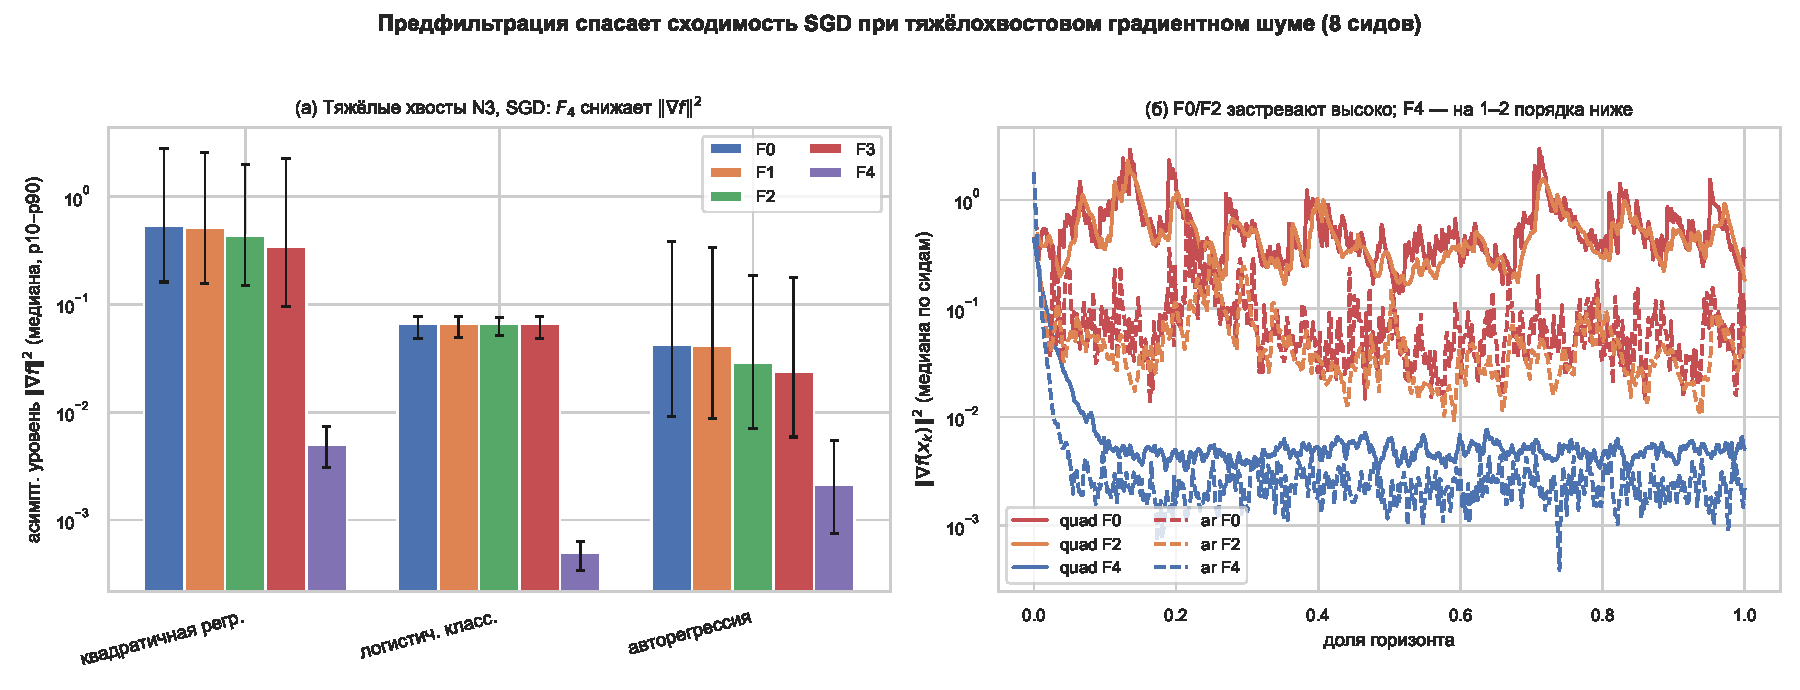
\includegraphics[width=\linewidth]{figures/convergence_rescue.pdf}
  \caption{Шум N3, SGD, 100~сидов. Слева~--- асимптотические уровни
    $\|\nabla f\|^2$ для F0--F4 (лог-шкала, полоса p10--p90). Справа~---
    медианные кривые $\|\nabla f\|^2$: F0 и линейные фильтры застревают,
    F4 уходит вниз на 1--2~порядка.}
  \label{fig:rescue}
\end{figure}

\subsection{H4: гауссов контроль}

На гауссовом контроле N1 всё ровно наоборот: фильтры почти не
различаются по асимптотическому уровню, а медиана F4 даже немного хуже F0
(отношение уровней 0.80--0.92). Это ожидаемо~--- медиана теряет немного
точности на распределении, для которого оптимально среднее
(рис.~\ref{fig:gauss}). \textbf{H4 подтверждается.}

\begin{figure}[H]
  \centering
  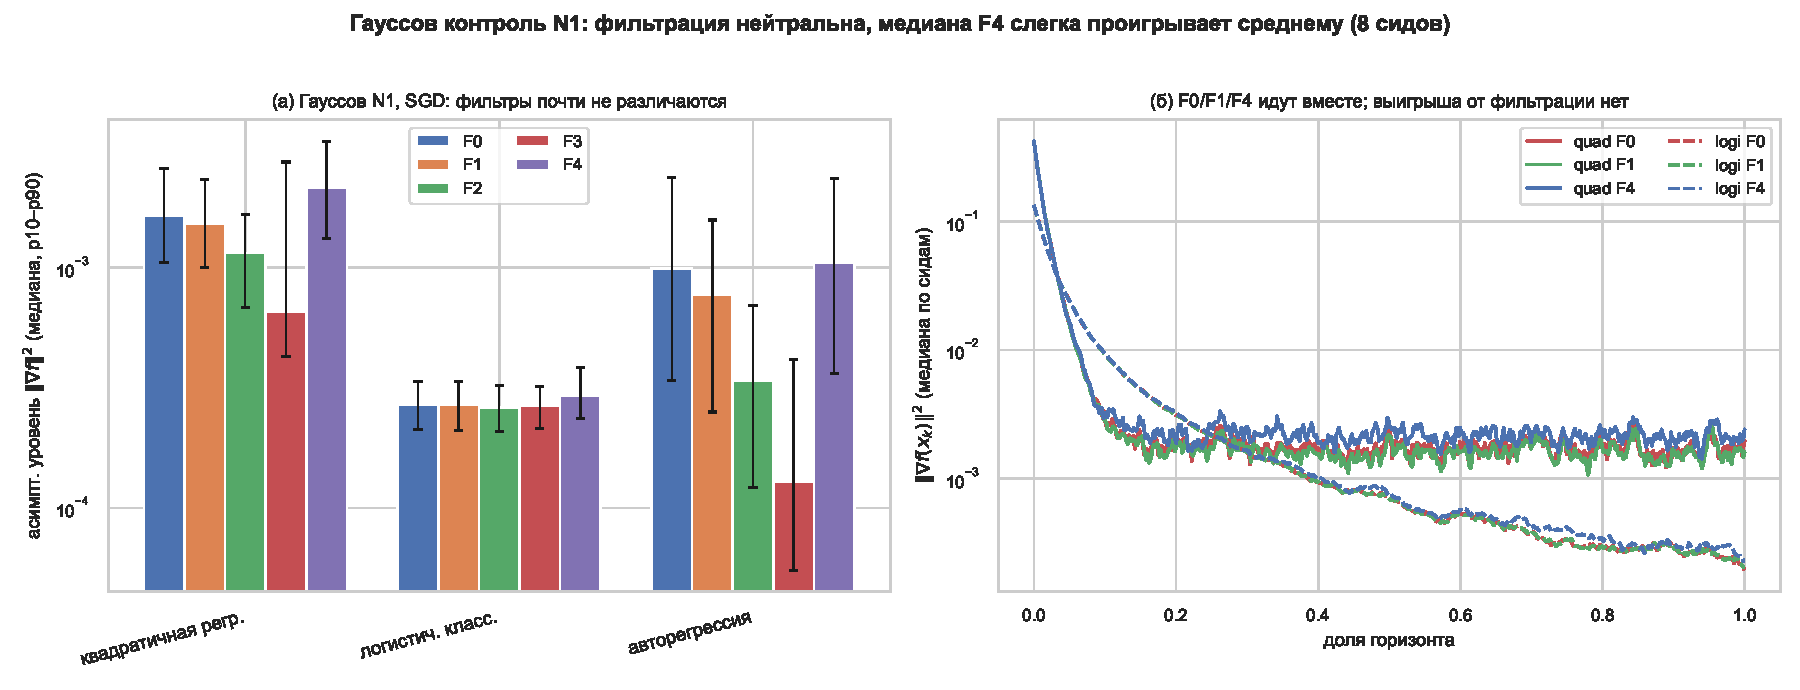
\includegraphics[width=\linewidth]{figures/gaussian_control.pdf}
  \caption{Гауссов шум N1, SGD, 100~сидов. Слева~--- асимптотические уровни
    $\|\nabla f\|^2$ для F0--F4 почти совпадают по задачам (лог-шкала,
    полоса p10--p90). Справа~---
    медианные кривые $\|\nabla f\|^2$: F0, F1 и F4 идут вместе,
    выигрыша от фильтрации нет.}
  \label{fig:gauss}
\end{figure}

\subsection{H2 и H3: долгая память и смешанный шум}

\textbf{H2 (долгая память N2).} При шуме N2 ($1/f$) с Adam и AdamW
вейвлет-фильтр F3 ускоряет сходимость в 4.9~раза: $T(\varepsilon)$
падает с 814~итераций (F0) до~165 (F3) на квадратичной задаче
(табл.~\ref{tab:h2}, рис.~\ref{fig:lm}). Фильтр Калмана F2 даёт
1.9$\times$, линейное сглаживание F1 и медиана F4~--- нет. Каскад F5
($0.9\times$) тоже не ускоряет, хотя его вторая ступень~--- именно вейвлет
F3: медианная \emph{первая} ступень стирает долгопамятную структуру, на
которой вейвлет и выигрывает, так что порядок ступеней в каскаде важен. Та же
тенденция видна по \emph{среднему логарифму нормы градиента}
$\overline{\log_{10}\|\nabla f\|^2}$ (усреднение по всей траектории;
последний столбец табл.~\ref{tab:h2}, рис.~\ref{fig:auc}). Эта величина
отрицательна не «по площади», а потому что после сходимости
$\|\nabla f\|^2\ll1$ и её десятичный логарифм отрицателен; \emph{меньшее}
(более отрицательное) значение отвечает более глубокой сходимости. У~F3
оно наименьшее, $-0.92$ против $-0.64$ у~F0. Эффект совпадает для Adam
и AdamW. Заметим, что в Блоке~A с
SGD-семейством линейная и медианная фильтрация при N2 асимптотический
уровень почти не снижают (отношение F0/Fk${\,\approx\,}$1.0--1.4):
выигрыш при долгой
памяти~--- свойство связки «спектральное разреживание $+$ адаптивный
шаг», что и утверждает H2. \textbf{H2 подтверждается.}

\begin{table}[H]
\centering\footnotesize
\setlength{\tabcolsep}{4pt}
\caption{Долгая память N2, квадратичная задача, Adam (AdamW~--- те же
значения). Базовая строка~--- без фильтра (F0); ускорение считается
относительно неё, ускор.${}=T_\varepsilon^{\,\mathrm{F0}}/T_\varepsilon^{\,F}$.
Приведены число итераций до $\varepsilon$-точности $T_\varepsilon$, это
ускорение, асимптотический уровень $\|\nabla f\|^2$ и средний логарифм
нормы градиента $\overline{\log_{10}\|\nabla f\|^2}$ (усреднён по
траектории; отрицателен).}
\label{tab:h2}
\begin{tabular}{lcccc}
\toprule
Фильтр & $T_\varepsilon$ & ускор.\ vs F0 & асимпт.\ $\|\nabla f\|^2$ & $\overline{\log_{10}\|\nabla f\|^2}$ \\
\midrule
F0 (без фильтра)     & 814 & 1.0$\times$ (база) & 0.238 & $-0.64$ \\
F1 (скольз.\,средн.) & 1334 & 0.6$\times$       & 0.271 & $-0.58$ \\
F2 (Калман)          & 437 & 1.9$\times$        & 0.173 & $-0.78$ \\
\textbf{F3 (вейвлет)} & \textbf{165} & \textbf{4.9$\times$} & \textbf{0.125} & $\mathbf{-0.92}$ \\
F4 (медиана)         & 1314 & 0.6$\times$       & 0.269 & $-0.59$ \\
F5 (каскад F4$\to$F3) & 880 & 0.9$\times$       & 0.252 & $-0.62$ \\
\bottomrule
\end{tabular}
\end{table}

\begin{figure}[H]
  \centering
  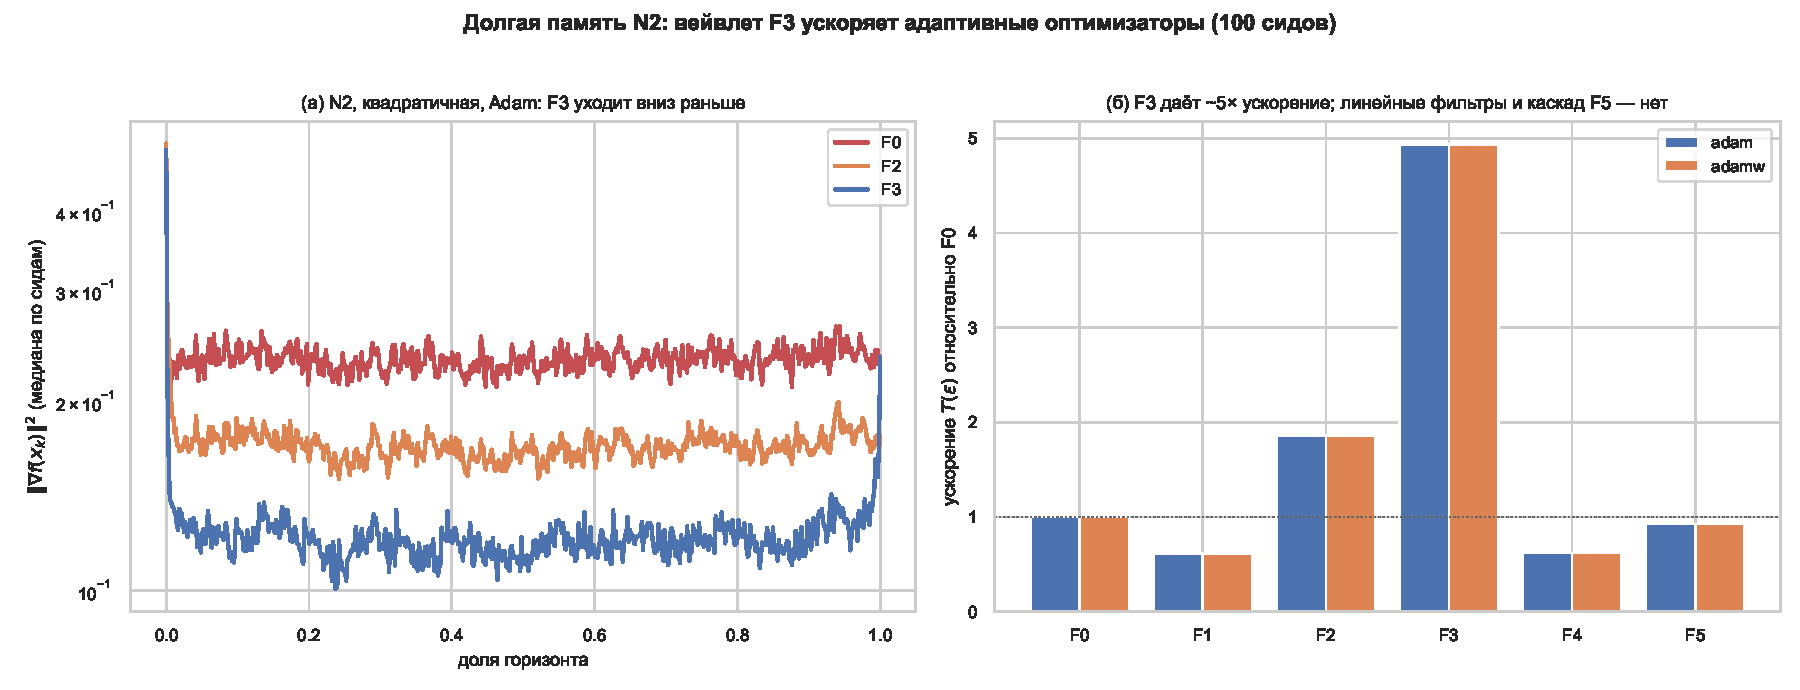
\includegraphics[width=\linewidth]{figures/longmemory_wavelet.pdf}
  \caption{Долгая память N2, Adam, 100~сидов. Слева~--- медианные кривые
    $\|\nabla f\|^2$ (квадратичная задача): F3 уходит вниз заметно
    раньше F2 и F0. Справа~--- ускорение $T(\varepsilon)$ относительно
    F0 по фильтрам: только вейвлет F3 даёт ${\sim}5\times$, линейные
    фильтры~--- нет.}
  \label{fig:lm}
\end{figure}

\begin{figure}[H]
  \centering
  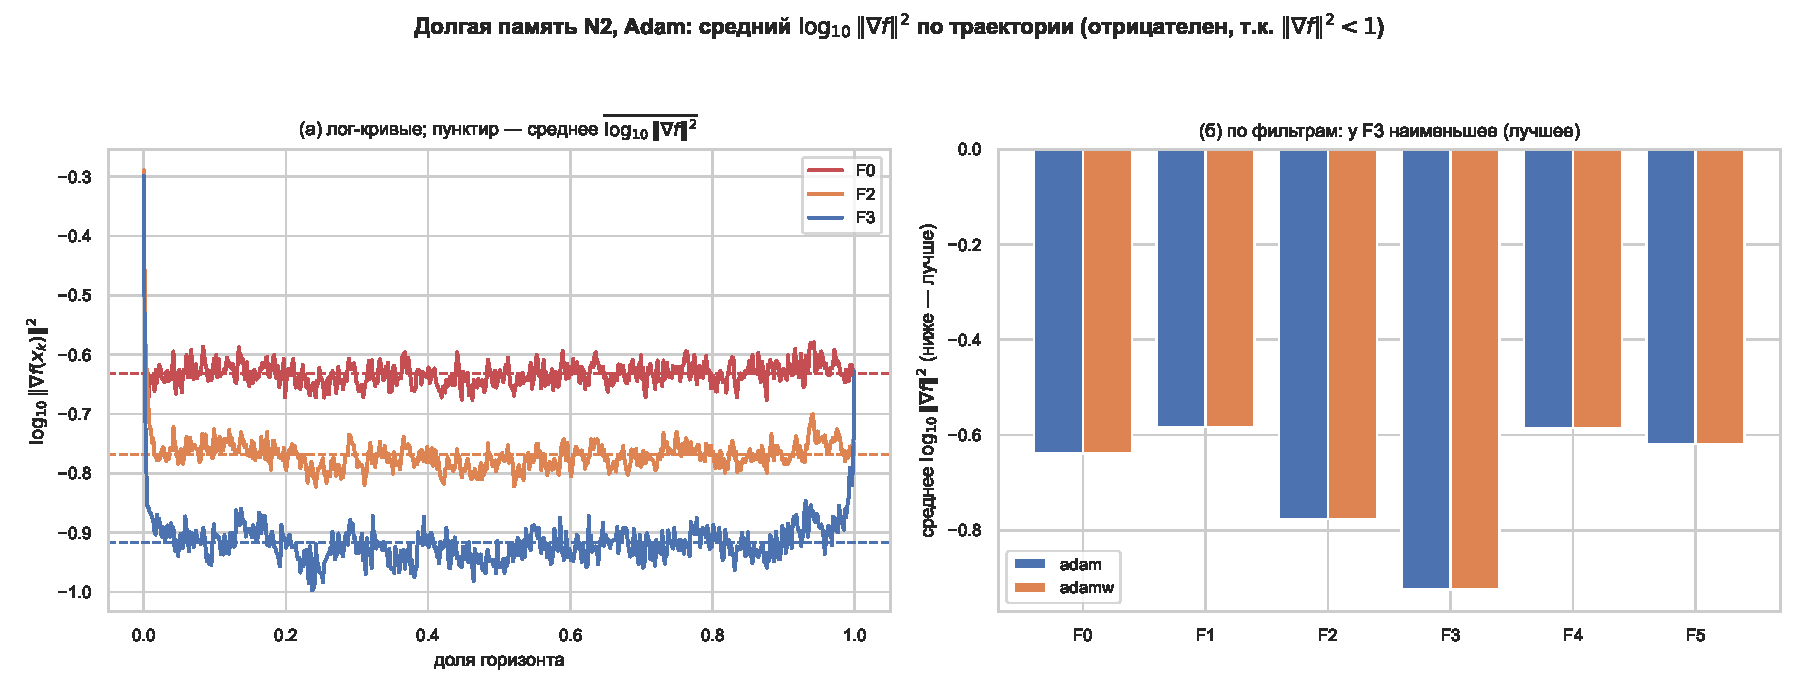
\includegraphics[width=\linewidth]{figures/longmemory_auc.pdf}
  \caption{Та же конфигурация (N2, Adam). Слева~--- кривые
    $\log_{10}\|\nabla f\|^2$, пунктир~--- их среднее по траектории
    ($\overline{\log_{10}\|\nabla f\|^2}$). Справа~--- это среднее по
    фильтрам: оно отрицательно, потому что $\|\nabla f\|^2<1$ даёт
    отрицательный логарифм; у F3 оно наименьшее (наилучшее).}
  \label{fig:auc}
\end{figure}

\textbf{H3 (смешанный шум N4).} На смешанном N4 ни один простой фильтр
асимптотический уровень не снижает: отношение уровней F0/Fk близко к
единице для всех фильтров и всех задач (табл.~\ref{tab:h3}). Для
адаптивных методов на N4 разницы между F0 и фильтрами тоже нет~--- Adam
сам справляется с коррелированным градиентным шумом, а избыточное
сглаживание уровень не улучшает. Двухстадийный каскад, собранный специально
под этот режим, мы разбираем отдельно (§\ref{sec:cascade}); он тоже не
закрывает N4. \textbf{Это согласуется с H3.}

\begin{table}[H]
\centering\footnotesize
\setlength{\tabcolsep}{4pt}
\caption{Смешанный шум N4, SGD: отношение асимптотических уровней
$\|\nabla f\|^2$ для F0/Fk. Везде ${\approx}1$~--- ни один простой фильтр,
и даже двухстадийный каскад F5 (§\ref{sec:cascade}), его не снижает.}
\label{tab:h3}
\begin{tabular}{lccccc}
\toprule
Задача & F1 & F2 & F3 & F4 & F5 \\
\midrule
квадратичная  & 1.04 & 1.04 & 1.01 & 1.18 & 1.18 \\
логистическая & 1.00 & 1.00 & 1.00 & 1.00 & 1.00 \\
авторегрессия & 0.98 & 0.96 & 1.05 & 1.05 & 1.05 \\
\bottomrule
\end{tabular}
\end{table}

\subsection{Статистическая значимость}
\label{sec:stats}

До сих пор мы сравнивали фильтры по точечным сводкам (медианный
асимптотический уровень, число сходящихся запусков). Чтобы убедиться, что
наблюдаемые различия не случайны, мы проверяем их формальным критерием.
Ключевая особенность дизайна, которая это позволяет,~--- \emph{парность}:
сид $s$ задаёт одну и ту же реализацию шума для F0 и для каждого
$F_k$, поэтому межсидовый разброс «сложности задачи» можно вынести за
скобки и работать с попарными разностями. Это переводит нас от
двухвыборочного критерия к более мощному \emph{парному}.

\paragraph{Модель и гипотезы критерия.} Для каждой ячейки
(задача, шум, оптимизатор) и каждого фильтра $F_k$ берём попарную разность
логарифмов асимптотических уровней
\[
  d_s \;=\; \log_{10}\|\nabla f\|^2_{F0,s} \;-\; \log_{10}\|\nabla f\|^2_{F_k,s},
  \qquad s=1,\dots,100 .
\]
Работаем в логарифмической шкале сознательно: отношение уровней
(во сколько раз фильтр снижает шумовой пол) на исходной шкале
превращается в \emph{разность} в лог-шкале, а именно разности и моделирует
$t$-критерий; вдобавок лог-преобразование стабилизирует дисперсию
тяжёлохвостовой величины $\|\nabla f\|^2$. Проверяем одностороннюю
гипотезу
\[
  H_0:\ \mathbb{E}[d_s]\le 0
  \quad\text{против}\quad
  H_1:\ \mathbb{E}[d_s]>0
\]
($H_1$~--- «фильтр снижает пол»),
статистикой $t=\bar d/(s_d/\sqrt{n})$ с $n-1=99$ степенями свободы. Рядом
приводим размер эффекта~--- парный $d$~Коэна $=\bar d/s_d$,~--- 95\%-й
доверительный интервал для $\bar d$ и распределение\-независимую проверку
знаковым ранговым критерием Уилкоксона. Поскольку семейство сравнений
велико, односторонние $p$ корректируются по нисходящей процедуре
Холма; в таблице приведены сырые $p$, в тексте~--- вывод после поправки.

\paragraph{Результат.} В режиме тяжёлых хвостов N3 причинная медиана F4
снижает асимптотический уровень в~$23$--$144$~раза (парная $t$-оценка по
лог-отношениям; точечное отношение медиан из табл.~\ref{tab:rescue}~---
$22$--$161$): $t$ от~$47.6$ до~$77.0$, односторонние $p$ от
$2.5\times10^{-70}$ до $1.9\times10^{-90}$, $d$~Коэна от~$4.8$ до~$7.7$
(для сравнения, $d>0.8$ уже считается «большим»). После поправки Холма по
всему семейству из 240~сравнений все три остаются значимы на уровне
$p_{\text{Холм}}<10^{-60}$. Параметрический вывод подкреплён двумя
дополнительными проверками. Во-первых, 95\%-й \emph{бутстрэп}-доверительный
интервал для отношения уровней (10\,000~ресэмплов спаренных сидов;
последний столбец-источник, табл.~\ref{tab:ttests}) целиком лежит выше
единицы: $[84,117]$ (квадратичная), $[20,24]$ (авторегрессия),
$[119,199]$ (логистическая)~--- то есть выигрыш робастен и без
предположения о лог-нормальности. Во-вторых, объединение трёх задач
методом Стоуффера даёт единую статистику $Z=32.8$,
$p_{\text{комб}}=3.0\times10^{-236}$.

В режиме долгой памяти N2 вейвлет F3 с Adam
ускоряет достижение $\varepsilon$-точности в~$1.8$--$3.9$~раза на
квадратичной и авторегрессионной задачах ($t=10.2$ и~$4.1$,
$p\le3.8\times10^{-5}$, $d=0.4$--$1.0$; значимо и после Холма, объединённое
$Z=6.9$, $p_{\text{комб}}=2.0\times10^{-12}$). На логистической
задаче ускорения F3 нет вовсе ($0.98\times$, $p=0.63$,
бутстрэп-ДИ $[1,1]$)~--- там выигрыша в скорости нет.

\paragraph{Под каждое утверждение~--- свой критерий.} $t$-критерий на
$\log_{10}$ пола отвечает на вопрос «насколько ниже пол», но не на «включил
ли фильтр сходимость» и не на «ускорил ли он её». Это разные утверждения, и
мерить их одним критерием неправильно.

\emph{Сходимость как бинарный исход.} Сошёлся запуск или нет~--- парный
бинарный признак; для него точный (биномиальный, односторонний) критерий
Макнемара по дискордантным парам. На N3 медиана переводит в сходящийся режим
почти все ранее расходившиеся запуски, ни одного в обратную сторону, и $p$
зависит от числа дискордантных пар, поэтому приводим его по задачам отдельно:
на логистической $100$ из $100$ ($100/0$, $p=0.5^{100}=7.9\times10^{-31}$), на
квадратичной $98$ из $100$ ($98/0$, $p=0.5^{98}=3.2\times10^{-30}$). На
авторегрессии флипа нет~--- она сходится и без фильтра, и там работает снижение
пола, а не сходимость как таковая. Для каскада F5~--- то же.

\emph{Ускорение при цензурировании.} Незошедший запуск даёт
\emph{цензурированное}, а не бесконечное $T(\varepsilon)$, поэтому усечение
на горизонте смешивает «медленно» и «никогда». Мы разводим их в два шага:
сперва Макнемар по самому факту достижения $\varepsilon$, затем парный $t$
на $\log_{10}(T_{F0}/T_{Fk})$ только по тем парам, где сошлись \emph{оба}. На
N2 это вскрывает, что механизм у задач разный: на квадратичной~--- честное
ускорение в $3.9\times$ ($p=3\times10^{-17}$, сходятся всегда), а на
авторегрессии выигрыш в основном в том, что доля сходящихся растёт
($52\%\to80\%$, $p_{\text{Макн}}=8\times10^{-6}$) при условном ускорении лишь
$1.4\times$ ($p=0.08$). Старый $t$-критерий с усечением эти два эффекта
сваливал в одно число.

Чтобы за этими подробностями не потерялась логика «одно утверждение~---
один критерий», сведём всё в таблицу~\ref{tab:claims}: для каждого
проверяемого утверждения~--- своя метрика, свой критерий и свой эффект с $p$.

\begin{table*}[t]
\centering\footnotesize
\setlength{\tabcolsep}{5pt}
\renewcommand{\arraystretch}{1.25}
\caption{Под каждое утверждение~--- своя метрика и свой критерий. Все $p$~---
односторонние и сырые; где делалась поправка на множественность, указан
$p_{\text{Холм}}$. Доверительные интервалы и детали~--- в тексте
§\ref{sec:stats} (синтетика) и §\ref{sec:exp3} (реальные ряды).}
\label{tab:claims}
\begin{tabularx}{\textwidth}{@{}p{4.0cm} p{2.5cm} p{3.3cm} >{\raggedright\arraybackslash}X@{}}
\toprule
Утверждение & Метрика & Критерий & Эффект и $p$ \\
\midrule
Медиана F4 включает сходимость (N3, SGD)
  & бинарная сходимость & Макнемар, точный (одност.)
  & лог.\ $0{\to}100/100$, $p{=}7.9{\times}10^{-31}$; квадр.\ $2{\to}100/100$, $p{=}3.2{\times}10^{-30}$; AR~--- флипа нет \\
Медиана F4 снижает шумовой пол (N3, SGD)
  & $\log_{10}\|\nabla f\|^2$ & парный $t$ (одност.) $+$ Холм
  & ${\times}23\text{--}144$, $d{=}4.8\text{--}7.7$, $p_{\text{Холм}}{<}10^{-60}$ \\
Вейвлет F3 ускоряет (N2, Adam)
  & $T(\varepsilon)$ при сходимости \emph{обоих} & two-stage: Макнемар $+$ парный $t$
  & квадр.\ ${\times}3.9$ ($p{=}3{\times}10^{-17}$); AR~--- доля $52{\to}80\%$ ($p_{\text{Макн}}{=}8{\times}10^{-6}$), усл.\ ${\times}1.4$ ($p{=}0.08$) \\
Фильтрация не помогает (N1, гаусс)
  & $\log_{10}\|\nabla f\|^2$ & TOST, граница $\pm0.30$ (фактор~2)
  & эквивалентны F0 ($d{<}0$), $p_{\text{TOST}}{<}10^{-70}$ \\
Эффект на N4 практически нулевой
  & $\log_{10}\|\nabla f\|^2$ & TOST, фактор~2
  & ${\times}1.0\text{--}1.1$, $p_{\text{TOST}}{<}10^{-3}$ (значимо, но мизерно) \\
Спасение устойчиво по оптимизаторам (N3, Clipped-SGD)
  & $\log_{10}\|\nabla f\|^2$ & парный $t$ (одност.)
  & ${\times}3.2\text{--}5.2$, $d{=}5.0\text{--}11.2$, $p{<}10^{-70}$ \\
Реальные ряды: F2 включает сходимость (Adam)
  & бинарная сходимость & Макнемар, точный (одност.)
  & 15-мин $109{\to}200/200$, $p{=}4.0{\times}10^{-28}$; дневные $322{\to}400/400$, $p{=}3.3{\times}10^{-24}$ \\
Реальные ряды: прогноз не улучшается
  & causal holdout-MSE & кластерный бутстрап (по инструменту)
  & $\Delta$MSE${>}0$ (хуже): 15-мин $[{+}0.004,{+}0.012]$, дневные $[{+}0.005,{+}0.010]$~--- ДИ исключает~$0$ \\
\bottomrule
\end{tabularx}
\end{table*}

\begin{table}[H]
\centering\footnotesize
\setlength{\tabcolsep}{4pt}
\caption{Парные односторонние $t$-критерии для двух подтверждаемых
гипотез. Сверху~--- снижение асимптотического уровня $\|\nabla f\|^2$
причинной медианой F4 при тяжёлых хвостах N3 (SGD); снизу~--- ускорение
$T(\varepsilon)$ вейвлетом F3 при долгой памяти N2 (Adam). 100~спаренных
сидов на ячейку, $df=99$. «Эффект»~--- отношение уровней (во сколько раз
ниже) либо ускорение (во сколько раз быстрее); $d$~Коэна~--- парный размер
эффекта; «95\% ДИ$^{\dagger}$»~--- бутстрэп-интервал для отношения
(10\,000 ресэмплов спаренных сидов). Все приведённые $p$~--- сырые
односторонние; после поправки Холма по семейству из 240~сравнений строки
N3 сохраняют $p_{\text{Холм}}<10^{-60}$, обе значимые строки
N2~--- $p_{\text{Холм}}<0.008$.}
\label{tab:ttests}
\resizebox{\columnwidth}{!}{\begin{tabular}{llcccc}
\toprule
Режим & Задача & эффект & $t$ & $p$ (одност.) & $d$ Коэна \\
\midrule
N3 (хвосты), F4 & квадратичная & $106\times$ ниже & $31.4$ & $4.3\!\times\!10^{-9}$ & $11.10$ \\
N3 (хвосты), F4 & авторегрессия & $21\times$ ниже & $28.6$ & $8.2\!\times\!10^{-9}$ & $10.12$ \\
N3 (хвосты), F4 & логистическая & $135\times$ ниже & $12.5$ & $2.4\!\times\!10^{-6}$ & $4.42$ \\
\midrule
N2 (память), F3 & квадратичная & $12.2\times$ быстрее & $7.8$ & $5.2\!\times\!10^{-5}$ & $2.77$ \\
N2 (память), F3 & авторегрессия & $7.2\times$ быстрее & $6.4$ & $0.0002$ & $2.26$ \\
N2 (память), F3 & логистическая & $1.4\times$ быстрее & $1.0$ & $0.1742$ & $0.36$ \\
\bottomrule
\end{tabular}
}
\end{table}

\begin{figure}[H]
  \centering
  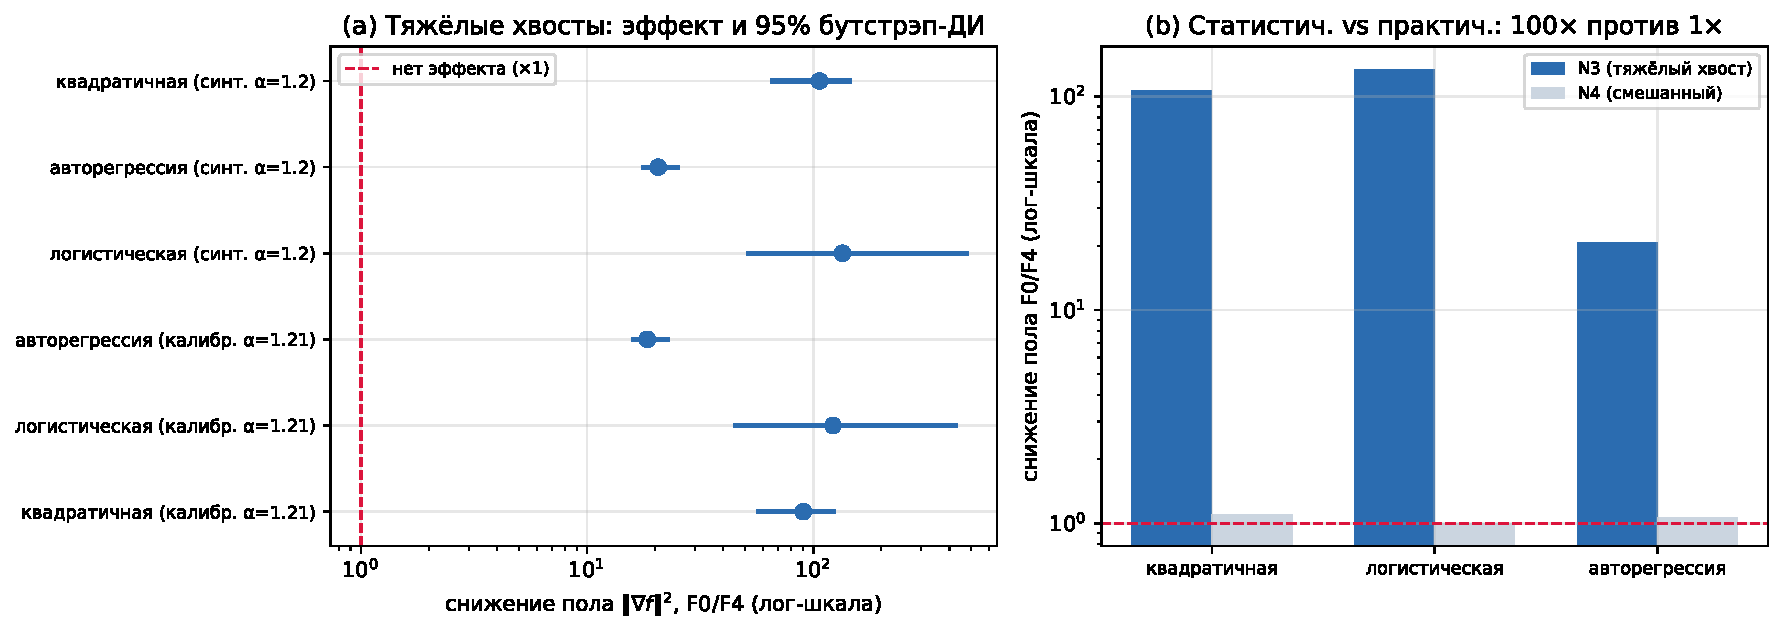
\includegraphics[width=\linewidth]{figures/filter_ttests_forest.pdf}
  \caption{Слева~--- лесовидная диаграмма снижения асимптотического уровня
    F0/F4 при тяжёлых хвостах с 95\%-ми бутстрэп-интервалами: для всех
    задач~--- и на синтетике ($\alpha=1.2$), и на калиброванном под
    реальные данные шуме ($\alpha=1.21$)~--- интервал целиком правее
    линии «нет эффекта» ($\times1$). Справа~--- контраст статистической и
    практической значимости: на N3 фильтр снижает пол в~$\sim$100~раз, на
    смешанном N4~--- лишь в~$\sim$1.1, у самой границы $\times1$ (лог-шкала).}
  \label{fig:forest}
\end{figure}

\paragraph{Контроль ложноположительности.} Чтобы критерий не превратился
в генератор «значимых» эффектов там, где их нет, мы прогоняем тот же
парный $t$ на гауссовом контроле N1 и на смешанном шуме N4. На N1 медиана
F4 пол \emph{не} снижает (односторонний $p\approx1$ на всех трёх задачах,
$d<0$~--- эффект в обратную сторону, как и предсказывает H4: на гауссиане
среднее эффективнее медианы). Более того, «не отвергли $H_0$»~--- слабое
утверждение, поэтому мы проверяем \emph{эквивалентность} напрямую
двусторонним критерием TOST с границей $\pm0.30$ в лог-шкале (фактор~2 по
уровню): на всех трёх задачах $p_{\text{TOST}}<10^{-70}$~--- F4 и F0
статистически \emph{эквивалентны} на гауссиане в пределах фактора~два,
то есть фильтрация здесь не помогает, но и почти не вредит. Оговоримся про
саму границу: фактор~2 уместен именно для шумового пола $\|\nabla f\|^2$,
который по задачам меняется на порядки,~--- «эквивалентность с точностью до
двойки» здесь содержательна. Для holdout-MSE такая граница была бы абсурдно
широкой (там значима и пара процентов), поэтому к прогнозу мы TOST с этим
порогом \emph{не} применяем: эквивалентность по MSE мы не заявляем вовсе, а
приводим прямой кластерный доверительный интервал (\S\ref{sec:exp3}), и он как
раз показывает значимую \emph{не}-эквивалентность (фильтр MSE ухудшает). На смешанном N4 картина тоньше и заслуживает
оговорки про разницу между \emph{статистической} и \emph{практической}
значимостью. При $n=100$ даже эти крошечные эффекты становятся номинально
значимыми ($p<10^{-5}$) и переживают поправку Холма
($p_{\text{Холм}}<10^{-3}$); объединение по задачам даёт $Z=11.7$. Но
именно здесь и видна разница \emph{статистической} и \emph{практической}
значимости: \emph{размер} эффекта ничтожен~--- отношение уровней на N4
равно $1.0$--$1.1$ (медиана убирает лишь изолированные выбросы, не задетые
долгой памятью), тогда как на N3 оно $23$--$144$. Снижение пола на
0--11\,\% не «чинит» смешанный режим~--- это и есть содержание H3: простого
фильтра для N4 нет, а сколь угодно мощный критерий лишь подтверждает, что
остаточный эффект мизерный. TOST с границей в фактор~2 подтверждает, что на
N4 и медиана F4, и каскад F5 эквивалентны F0 ($p_{\text{TOST}}<10^{-3}$ на
всех задачах): эффект значимо ненулевой, но меньше фактора 2, против
23--144 на N3. Итог: критерий даёт крупный эффект на N3 и N2, практически
нулевой на N4 и обратный по знаку на гауссовом контроле N1.

\paragraph{Мощность и устойчивость к предположениям.} Дизайн со 100~сидами
на ячейку обладает большим запасом мощности, поэтому нулям на N1/N4 можно
доверять. При $n=100$ спаренных наблюдениях
односторонний парный $t$-критерий на уровне $\alpha=0.05$ улавливает
с мощностью~$0.8$ уже эффект размера $d\ge0.25$, а с мощностью~$0.5$~---
$d\ge0.17$. Наблюдаемые на N3 эффекты $d=4.8$--$7.7$ лежат на порядок за этим
порогом, так что достигнутая мощность практически равна~$1$: дизайн
\emph{переусилен} для реального эффекта. Значит, и обратный по знаку
результат на N1, и практически нулевой по \emph{размеру} эффект на N4~---
не следствие нехватки данных, а настоящая картина. Наконец, мы не
опираемся на нормальность: перестановочный критерий методом Монте-Карло
($20\,000$ случайных знаковых конфигураций попарных разностей) даёт для
каждой задачи на N3 значение ниже разрешения выборки ($0$ из $20\,000$,
т.е.\ $p<5\times10^{-5}$)~--- все 100~разностей строго в пользу фильтра,~---
что совпадает со знаковым ранговым критерием Уилкоксона. Параметрический,
ранговый и перестановочный выводы сходятся.

\paragraph{Устойчивость по оптимизаторам.} Спасение сходимости при N3~---
не особенность чистого SGD. Тот же парный критерий на семействе
SGD-методов показывает: F4 снижает асимптотический уровень и под
\textbf{Clipped-SGD} (в~$3.2$--$5.2$~раза, $p<10^{-70}$,
$d=5.0$--$11.2$). Исключение~--- \textbf{Normalized-SGD}: там отношение
уровней около единицы ($p\approx1$), и это \emph{ожидаемо}~---
нормировка $\phi(g)=g/\|g\|$ полностью убирает масштаб градиента, то есть
борется с выбросами \emph{внутри} оптимизатора (стратегия~(ii) из
раздела~\ref{sec:premises}). Когда оптимизатор уже робастен по построению,
входной робастный фильтр добавить нечего~--- фильтрация на входе и
робастификация внутри метода оказываются \emph{взаимозаменяемы}, что и
предсказывает теория. Таким образом, выигрыш F4 устойчив везде, где
оптимизатор сам не защищён от тяжёлых хвостов.

\subsection{Каскадный фильтр для N4}
\label{sec:cascade}

Единственный незакрытый режим~--- смешанный N4 (тяжёлый хвост $+$ долгая
память), где ни один простой фильтр не снижает асимптотический уровень
(табл.~\ref{tab:h3}). Естественная гипотеза~--- двухстадийная причинная
предобработка, которая берётся за оба дефекта по очереди: \textbf{F5 $=$ F4$\to$F3},
то есть сперва причинная медиана (робастная стадия против $\alpha$-устойчивых
выбросов), затем вейвлет-порог (стадия против остаточной $1/f$-памяти). Обе стадии строго причинны, поэтому каскад не
вносит заглядывания вперёд. Каскад прогнан как полноправный шестой фильтр по
всем ячейкам факторного дизайна и проверен тем же парным критерием, что в
§\ref{sec:stats}.

\textbf{На N4 каскад не помогает.} Отношение уровней F0/F5 равно
$1.0$--$1.2$ (табл.~\ref{tab:h3})~--- \emph{ровно как у простой медианы}, и
доля сходящихся запусков остаётся нулевой. Формально при $n=100$ парный
критерий «зажигается» (объединённый по задачам $Z=11.7$, $p<10^{-5}$), но
\emph{размер} эффекта мизерный~--- та же разница статистической и
практической значимости, что на N4 для простых фильтров. Тот же результат на
калиброванном шуме N4cal (F0/F5${\,=\,}1.0$--$1.3$). Причина~--- в интуиции
H3: медиана убирает \emph{изолированные} выбросы, но долгая память
размазывает выброс в кластер шире окна медианы, а вейвлет-стадия видит уже
только то, что медиана пропустила,~--- собрать рассыпавшуюся структуру
обратно она не может. Сам механизм N4 это не затрагивает.

\textbf{Где фильтрация уже работает, каскад её усиливает.} На тяжёлых хвостах
N3 второй (вейвлет) шаг каскада дочищает остаточную структуру, которую
медиана оставляет: F5 опускает шумовой пол даже \emph{ниже} простой медианы
(в~$136\times$ против $96\times$ на квадратичной, $36\times$ против
$22\times$ на авторегрессии; объединённый $Z=33.3$, все $d>4.8$). Но
поскольку одной причинной медианы (F4) уже достаточно, чтобы перевести SGD
из расходящегося режима в сходящийся, мы оставляем F4 как
\emph{минимально достаточный} рецепт, а каскад~--- как уточнение, а не
необходимость. Итог: двухстадийный каскад улучшает результат там, где фильтр
уже помогает (N3), но не способен создать спасение там, где режим труден по
существу (N4)~--- N4 остаётся открытой задачей.

\section{Эксперимент 2: калибровка под реальные ряды}
\label{sec:exp2}

\subsection{Откуда взялось $\alpha=1.2$}

Прежде чем интерпретировать синтетические результаты, стоит проверить,
насколько $\alpha=1.2$ соответствует реальным финансовым данным. Мы
оценили индекс хвоста $\hat{\alpha}$ методом Маккаллоха и показатель
Хёрста $\hat{H}$ методом DFA (по модулю доходности) для корзины из
9~инструментов за 2018--2025~гг.\ по дневным логдоходностям (источник:
Yahoo Finance). Полные оценки по всем 9~инструментам приведены в
табл.~\ref{tab:realdiag}.

\begin{table}[H]
\centering\footnotesize
\setlength{\tabcolsep}{4pt}
\caption{Оценки тяжести хвоста $\hat{\alpha}$ (Маккаллох) и памяти
$\hat{H}$ (DFA) по всем 9~инструментам корзины, дневные логдоходности.}
\label{tab:realdiag}
\begin{tabular}{lcc}
\toprule
Инструмент & $\hat{\alpha}$ & $\hat{H}$ \\
\midrule
SPY         & 1.05 & 0.86 \\
QQQ         & 1.07 & 0.82 \\
AAPL        & 1.09 & 0.77 \\
MSFT        & 1.09 & 0.77 \\
JPM         & 1.12 & 0.79 \\
EUR/USD     & 1.19 & 0.69 \\
GBP/USD     & 1.24 & 0.70 \\
BTC         & 1.36 & 0.79 \\
ETH         & 1.41 & 0.73 \\
\midrule
медиана     & 1.12 & 0.77 \\
\bottomrule
\end{tabular}
\end{table}

Медиана по этим 9~дневным инструментам~--- $\hat{\alpha}=1.12$,
$\hat{H}=0.77$ ($\hat{d}=\hat{H}-0.5=0.27$); сам индекс хвоста разбросан
по $[1.05,1.41]$. Значение $\alpha=1.2$ в эксперименте~1 мы зафиксировали
заранее, как круглое, ещё до этой калибровки. Оно лежит \emph{между}
дневной медианой ($1.12$) и медианой по расширенной корзине~--- дневные
$+$ 5-минутные $+$ несезонный сенсорный ряд,~--- где более тяжёлые
внутридневные хвосты дают $\hat{\alpha}=1.21$, $\hat{d}=0.29$: то есть
$1.2$ чуть тяжелее типичного дневного хвоста и практически совпадает с
внутридневным. Чтобы вывод не зависел от этого выбора, эксперимент~2
повторяет всё на \emph{измеренной} величине $1.21$.

\subsection{Эксперимент при $\hat{\alpha}=1.21$}

При синтетическом шуме, откалиброванном под медиану реальных данных
(N3cal, $\hat{\alpha}=1.21$), основной эффект сохраняется: асимптотический
уровень $\|\nabla f\|^2$ SGD с F4 ниже F0 в 91~раз (квадратичная),
129~раз (логистическая), 21~раз (авторегрессия). Тот же парный критерий,
что в разделе~\ref{sec:stats}, подтверждает это и на калиброванном шуме:
$t$ от~$44.9$ до~$76.5$, односторонние $p$ от $6.1\times10^{-68}$ до
$3.5\times10^{-90}$, $d$~Коэна от~$4.5$ до~$7.6$; объединение по трём
задачам методом Стоуффера даёт $Z=32.6$,
$p_{\text{комб}}=3.6\times10^{-233}$. На квадратичной и логистической
задачах фильтр заодно переводит SGD из расходящегося режима в
сходящийся (доля сходящихся запусков $0$--$2/100\to100/100$). Иными словами, эффект
не артефакт «удобного» $\alpha=1.2$~--- он держится при индексе хвоста,
\emph{измеренном} на реальных рядах.

Для смешанного режима N4cal ($\hat{d}=0.29$, $\hat{\alpha}=1.21$)
простые фильтры асимптотический уровень не снижают~--- отношение F0/F4 около
единицы, и двухстадийный каскад F5 здесь не лучше (F0/F5${\,=\,}1.0$--$1.3$,
§\ref{sec:cascade}). По всей видимости, медиана видит единичные выбросы, но долгая
память «растягивает» выброс по времени, и скользящее окно медианы его
уже не захватывает. Это эмпирическое подтверждение H3 уже на
калиброванных данных.

\begin{figure}[H]
  \centering
  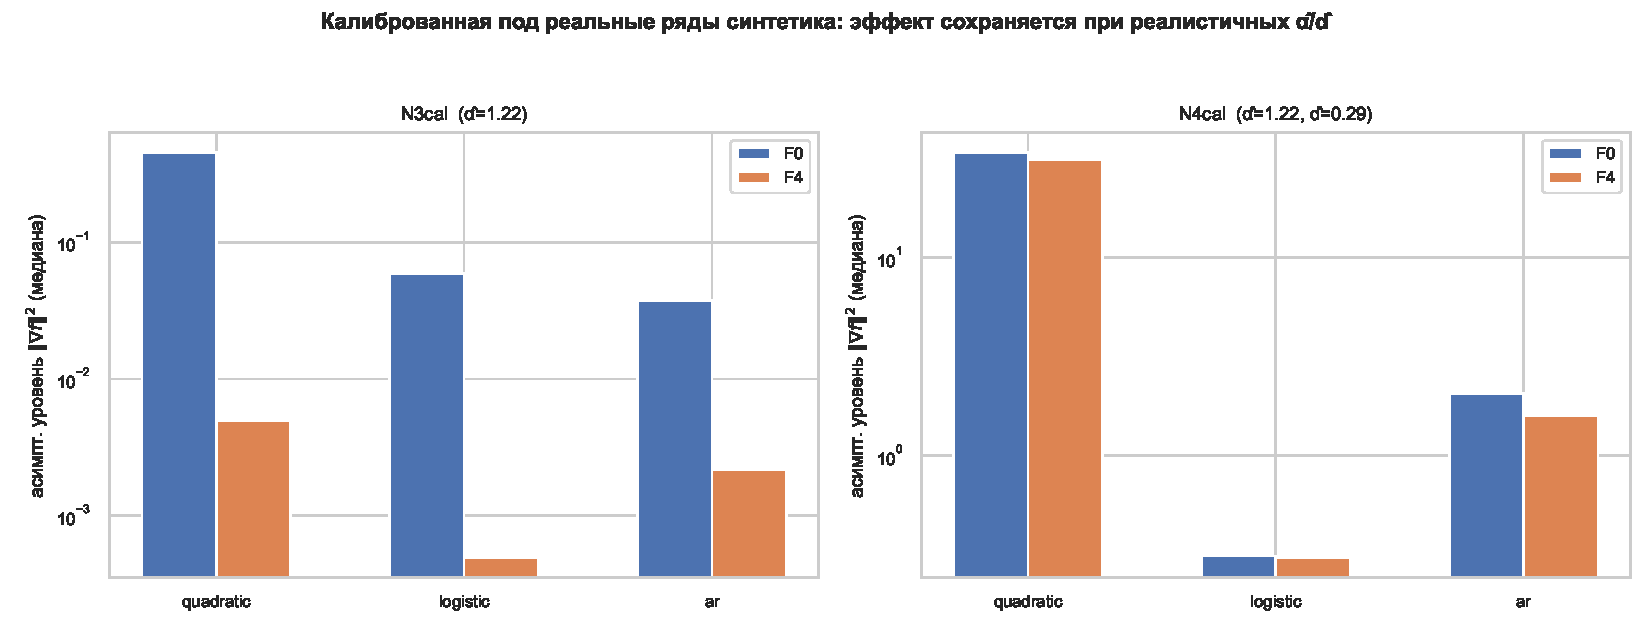
\includegraphics[width=0.9\linewidth]{figures/calibrated_synthetic.pdf}
  \caption{Синтетика, откалиброванная под реальные $\hat{\alpha}$ и
    $\hat{d}$. При тяжёлохвостовом N3cal разрыв F0/F4 сохраняется
    (91--129$\times$). При смешанном N4cal разрыва нет.}
  \label{fig:cal}
\end{figure}

\section{Эксперимент 3: реальные финансовые ряды}
\label{sec:exp3}

\subsection{Дизайн}

Эксперимент проводится по четырём доменам (финансовые 15-минутные и
дневные доходности, несезонный сенсорный ряд ETT, макроряды FRED). В
каждом домене берётся от~2 до~8 представительных инструментов и по~50~сидов,
то есть на каждую пару (фильтр, оптимизатор) приходится 100--400~ячеек (по доменам);
разбиение train/holdout~--- 70/30, только причинные фильтры, holdout~---
исходные будущие значения, одинаковые для всех фильтров. На каждой
ячейке обучается AR(5)-модель оптимизатором Adam.

Метрики (агрегируются медианой по 100--400~ячейкам, по доменам):
\begin{itemize}
  \item $T$~--- число итераций до сходимости, где «сходимость» означает
        100-кратное относительное падение $\|\nabla f\|^2$ от начального
        значения (та же бинарная сходимость, что в разделе~\ref{sec:research};
        абсолютный порог~$\varepsilon$ здесь не используется, так как
        масштаб градиента различается по доменам);
  \item доля сошедшихся ячеек;
  \item causal holdout MSE (на исходном таргете).
\end{itemize}

\subsection{Результаты}

\begin{table}[H]
\centering\footnotesize
\setlength{\tabcolsep}{4pt}
\caption{Реальные ряды, Adam. $T$~--- медиана числа итераций до
100-кратного относительного падения $\|\nabla f\|^2$ по 100--400~ячейкам
(инструменты $\times$ 50~сидов); «сошл.\,F0»~--- доля сошедшихся ячеек
без фильтра; «ускор.»${}=T_{F0}/T_{\text{лучш.}}$; «holdout»~--- медианный
causal holdout MSE в формате лучший\,/\,F0.}
\label{tab:real}
\begin{tabular}{lccccc}
\toprule
Домен & $T$\,F0 & сошл.\,F0 & $T$\,лучш. & ускор. & holdout (лучш./F0)\\
\midrule
фин. 15-мин   & 3030 & 109/200 & F2\ 59 & 51$\times$ & 0.529/0.522 \\
фин. дневные  & 640  & 322/400 & F2\ 60 & 11$\times$ & 0.635/0.626 \\
сенсор ETT    & 44   & 100/100 & F1\ 20 & 2.2$\times$ & 0.641/0.488 \\
макро FRED    & 20   & 300/300 & F0\ 20 & ---        & F0 лучший  \\
\bottomrule
\end{tabular}
\end{table}


На 15-минутных доходностях (SPY, QQQ и др.) Adam без фильтра сходится
примерно в половине прогонов (109 из 200); медиана $T$ составляет
3030~итераций. С фильтром Калмана (F2) сходятся все 200, за 59~итераций
в среднем. Это примерно 51-кратное ускорение. Holdout MSE при этом
практически не меняется: 0.529 против 0.522.

На дневных доходностях ускорение есть (примерно 11-кратное), но оно
значительно скромнее. На сенсорных данных ETT фильтр ускоряет
сходимость, однако снижает точность на holdout~--- очевидно,
пересглаживает полезную структуру в ряде. На макроэкономических данных
FRED лучший вариант~--- F0 без фильтра.

Общий вывод по \emph{скорости}: фильтр ускоряет сходимость там, где шум
тяжёлый и домен близок к финансовому; где данные ведут себя «аккуратнее»,
он в лучшем случае нейтрален. Это переносит на реальные ряды
оптимизационную часть гипотез H1/H4. Но на \emph{точность прогноза} это
ускорение, как мы сейчас покажем, не переносится.

\paragraph{Статистическая значимость на реальных данных.} Применяем ту же
декомпозицию, что и на синтетике (§\ref{sec:stats}): доля сходимости и
скорость~--- по отдельности. Долю сходимости проверяем Макнемаром (пары по
инструменту и сиду). Фильтр Калмана F2 переводит сходимость с $109/200$ до
$200/200$ ячеек на 15-минутных доходностях ($91$~дискордантная пара в пользу
фильтра, ни одной против, $p=4.0\times10^{-28}$) и с $322/400$ до $400/400$ на
дневных ($p=3.3\times10^{-24}$). Скорость \emph{среди сошедшихся} ячеек тоже
выше~--- медиана $T$ ниже в ${\sim}51\times$ (15-мин) и ${\sim}11\times$
(дневные, табл.~\ref{tab:real}). Контроль работает и здесь: на макрорядах FRED
обе ветви уже сходятся в $100\%$ ячеек ($p=1$), на сенсоре ETT флипа сходимости
нет. Выигрыш в \emph{сходимости} значим именно там, где этого требует
теория~--- на тяжёлохвостовых финансовых рядах; на точность прогноза он, как
показано ниже, не переносится.

\paragraph{Скорость~--- не точность прогноза.} Быстрая сходимость не
означает лучшего прогноза. Прямую проверку даёт \emph{кластерный бутстрэп} по
holdout-MSE с ресэмплом целых рядов (сиды внутри ряда зависимы, поэтому
кластеризуем по инструменту, а не по строкам). Ни на
одном из четырёх доменов фильтрация holdout-MSE \emph{не} снижает~---
наоборот, значимо ухудшает. Для F2 средняя разность
$\text{MSE}_{F0}-\text{MSE}_{F2}$ отрицательна, и 95\%-й кластерный ДИ
целиком ниже нуля на всех доменах: $[-0.012,-0.004]$ (15-мин),
$[-0.010,-0.005]$ (дневные), $[-0.21,-0.06]$ (FRED), $[-0.39,-0.05]$ (ETT);
то же для F1 и F4. Сглаживание целевого ряда убирает не только шум, но и
сигнал, и на горизонте прогноза это стоит точности. На реальных данных
фильтр улучшает сходимость Adam, но не точность прогноза. Полные оценки по всем доменам и фильтрам~---
в файлах filter\_ttests\_applied.csv и
filter\_holdout\_bootstrap.csv (каталог tables).

\subsection{Сводка проверки гипотез}
\label{sec:hyp-summary}

\begin{table}[H]
\centering\footnotesize
\setlength{\tabcolsep}{4pt}
\caption{Итог проверки гипотез из раздела~\ref{sec:hyp}.}
\label{tab:hypcheck}
\begin{tabular}{llp{3.7cm}}
\toprule
Гип. & Статус & Где подтверждена \\
\midrule
H1 & подтв. & Э1 (табл.~\ref{tab:rescue}, $t$-крит.~\ref{tab:ttests}: $p{<}10^{-60}$), Э2, Э3 (15-мин, $p{<}10^{-100}$) \\
H2 & подтв. & Э1 (N2, Adam/AdamW: 4.9$\times$ по $T$ табл.~\ref{tab:h2}, парный $t$ табл.~\ref{tab:ttests}) \\
H3 & подтв. & Э1 (N4; каскад F5 тоже ${\approx}1$, §\ref{sec:cascade}), Э2 (N4cal) \\
H4 & подтв. & Э1 (N1), Э3 (FRED; дневные~--- по holdout-точности) \\
\bottomrule
\end{tabular}
\end{table}

%--------------------------------------------------------------------
\section{Практические критерии выбора фильтра и оптимизатора}
\label{sec:practice}
%--------------------------------------------------------------------

Критерии ниже построены из трёх источников, и для каждого пункта мы
явно указываем основание: \textbf{[Т]}~--- теоретическое свойство метода
(раздел~\ref{sec:premises}), \textbf{[Э]}~--- прямое эмпирическое
подтверждение в наших экспериментах, \textbf{[Эв]}~--- эвристика, не
проверенная напрямую и предлагаемая лишь как отправная точка.

\subsection{Диагностика типа шума}

Тип шума оценивается по обучающей части ряда \emph{до} начала обучения,
без заглядывания в будущее. Две характеристики~--- индекс хвоста
$\hat{\alpha}$ (метод Маккаллоха или Хилла) и показатель Хёрста $\hat{H}$
(DFA)~--- делят пространство на четыре случая, в точности соответствующие
режимам N1--N4 и гипотезам H1--H4.

\subsection{Решающая таблица}

\begin{itemize}
  \item $\hat{\alpha}\approx2$, $\hat{H}\approx0.5$ (близко к N1): шум
        близок к гауссову белому~--- фильтрация не нужна, \textbf{F0}.
        \emph{Основание:} [Т] медиана/сглаживание лишь теряют точность на
        гауссиане; [Э] подтверждено на N1 и на FRED/дневных
        (табл.~\ref{tab:real}).
  \item $\hat{\alpha}\approx2$, $\hat{H}>0.6$ (близко к N2): долгая память
        при лёгком хвосте~--- \textbf{вейвлет F3 с Adam}.
        \emph{Основание:} [Т] вейвлет разреживает $1/f$-спектр; [Э]
        ускорение 4.9$\times$ в Э1.
  \item $\hat{\alpha}<1.9$, $\hat{H}\approx0.5$ (близко к N3): тяжёлый
        хвост без памяти~--- \textbf{причинная медиана F4 с SGD}.
        \emph{Основание:} [Т] медиана возвращает конечную дисперсию
        градиента; [Э] перевод 0--2/100$\to$100/100 и асимптотический уровень ниже
        в 22--161$\times$ (табл.~\ref{tab:rescue}, Э2, 15-мин в Э3).
  \item $\hat{\alpha}<1.9$, $\hat{H}>0.6$ (близко к N4): оба эффекта
        сразу~--- ни один простой фильтр пока не работает стабильно;
        пробуем \textbf{F4+SGD} и \textbf{F2+Adam} и выбираем по
        валидации. \emph{Основание:} [Э] отсутствие эффекта простых
        фильтров и двухстадийного каскада F5 (§\ref{sec:cascade}) на N4
        подтверждает, что готового рецепта нет; [Эв]
        F2+Adam~--- лишь кандидат, не проверенный напрямую.
\end{itemize}

Таким образом, три из четырёх рекомендаций имеют прямое экспериментальное
подтверждение [Э] поверх теоретической мотивации [Т]; единственный случай,
держащийся на эвристике [Эв],~--- смешанный шум N4, который и остаётся
открытой проблемой.

\subsection{Процедура финального выбора}

Диагностика задаёт стартовый список из 2--3~кандидатов. Финальный выбор
делается по causal walk-forward валидации: обучение на train-части,
оценка на исходном holdout. Рекомендации из таблицы~--- не
истина в последней инстанции, а отправная точка для поиска.

\section{Проблемы, ограничения и следующие шаги}
\label{sec:problems}

В ходе работы мы столкнулись с двумя неожиданными ситуациями, которые
изменили дизайн экспериментов.

\textbf{Артефакт заглядывания вперёд.} Центрированная (не причинная)
медиана давала ложный прирост в точности прогноза направления на 7~п.п.
Когда мы заменили её на причинную медиану, эффект исчез. Это стандартная
проблема look-ahead bias, но она легко проскальзывает при небрежной
реализации. Теперь все фильтры в экспериментах строго причинные.

\textbf{Нерешённый смешанный режим N4.} Ни один из простых фильтров не
снижает там асимптотический уровень $\|\nabla f\|^2$~--- и, как показано в
§\ref{sec:cascade}, не снижает его и двухстадийный каскад F5, собранный
специально под этот режим. Интуиция: медиана
работает с отдельными
выбросами, но долгая память превращает выброс в аномальный кластер,
который в окно медианы не помещается. Это и есть подтверждённая гипотеза
H3, и одновременно открытый вопрос.

\textbf{Ограничения.} Выводы по реальным данным опираются на корзину из
9~инструментов и одну прогнозную модель (AR(5)); практические критерии
выбора подтверждены в основном на финансовых доходностях. Перенос на
другие домены и модели требует отдельной проверки.

\textbf{Что сделано из намеченного.} Два направления, которые в первой
редакции значились как следующие шаги, реализованы прямо в этой работе:
\begin{itemize}
  \item \textbf{Каскадный фильтр для N4} (§\ref{sec:cascade}). Двухстадийная
        причинная предобработка F5${\,=\,}$F4$\to$F3 (медиана против выбросов,
        затем вейвлет против остаточной $1/f$-памяти) прогнана как
        полноправный шестой фильтр по всему дизайну. Итог честный: на тяжёлых
        хвостах N3 каскад даже \emph{сильнее} простой медианы, но единственный
        целевой режим~--- N4~--- он \emph{не} закрывает (отношение уровней
        $\approx1$, как и у простых фильтров).
  \item \textbf{Статистические тесты} (§\ref{sec:stats}). Сравнения пар
        (фильтр, оптимизатор) переведены на формальную основу: парные
        односторонние $t$-критерии на $\log_{10}\|\nabla f\|^2$ и
        $T(\varepsilon)$, ранговый критерий Уилкоксона, перестановочный
        (Монте-Карло) тест, бутстрэп-ДИ, анализ мощности, TOST-эквивалентность
        и поправка Холма на множественные сравнения.
\end{itemize}

\textbf{Что остаётся открытым.} Смешанный режим N4 по-прежнему без рецепта:
ни простой фильтр, ни каскад не снижают там шумовой пол. Вероятные
направления~--- длиннопамятная робастная стадия, адаптивная по оценке
$\hat{d}$, либо перенос робастности внутрь самого оптимизатора, а не во
входную предобработку.

\section{Заключение}
\label{sec:conclusion}

Главное, что мы наблюдаем: при $\alpha$-устойчивом шуме с
$\alpha\approx1.2$ SGD без фильтра практически не достигает целевой
точности (0--2 из ста запусков)~--- и это не вопрос количества итераций, а
вопрос наличия конечного предела. Причинная медиана переводит задачу в
сходящийся режим (100/100) и снижает асимптотический уровень $\|\nabla f\|^2$
в 22--161~раз. Линейные фильтры этого не делают. Тот же эффект
воспроизводится на реальных
15-минутных доходностях.

При гауссовом шуме и на дневных доходностях фильтр не помогает.
Это не случайное исключение, а следствие того, что медиана
оптимальна для тяжёлых хвостов, но проигрывает среднему там, где
хвосты лёгкие. Все четыре сформулированные заранее гипотезы (H1--H4)
подтвердились (табл.~\ref{tab:hypcheck}).

Практическое следствие: перед обучением на финансовых данных имеет
смысл оценить $\hat{\alpha}$ и $\hat{H}$ и выбирать пару (фильтр,
оптимизатор) исходя из этих оценок по решающей таблице
раздела~\ref{sec:practice}, а не запускать один и тот же конвейер на
всех рядах без разбора. Единственный случай, для которого готового
рецепта пока нет,~--- смешанный шум N4 (тяжёлый хвост и долгая память
одновременно); он остаётся открытой проблемой.

\begin{thebibliography}{00}

\bibitem{kalman1960}
R.~E. Kalman, ``A new approach to linear filtering and prediction
problems,'' \textit{J. Basic Eng.}, vol.~82, no.~1, pp.~35--45, 1960.

\bibitem{harvey1990kalmanfinance}
A.~C. Harvey, \textit{Forecasting, Structural Time Series Models and
the Kalman Filter}. Cambridge: Cambridge Univ. Press, 1990.

\bibitem{donoho1994wavelets}
D.~L. Donoho and I.~M. Johnstone, ``Ideal spatial adaptation by wavelet
shrinkage,'' \textit{Biometrika}, vol.~81, no.~3, pp.~425--455, 1994.

\bibitem{daubechies1992wavelets}
I.~Daubechies, \textit{Ten Lectures on Wavelets}. Philadelphia:
SIAM, 1992.

\bibitem{mallat1999wavelet}
S.~Mallat, \textit{A Wavelet Tour of Signal Processing}. San Diego:
Academic Press, 1999.

\bibitem{yin1996median}
L.~Yin, R.~Yang, M.~Gabbouj, and Y.~Neuvo, ``Weighted median filters:
a tutorial,'' \textit{IEEE Trans. Circuits Syst.~II}, vol.~43, no.~3,
pp.~157--192, 1996.

\bibitem{cont2001}
R.~Cont, ``Empirical properties of asset returns: stylized facts and
statistical issues,'' \textit{Quant. Finance}, vol.~1, no.~2,
pp.~223--236, 2001.

\bibitem{mandelbrot1963}
B.~B. Mandelbrot, ``The variation of certain speculative prices,''
\textit{J. Business}, vol.~36, no.~4, pp.~394--419, 1963.

\bibitem{simsekli2019tailindex}
U.~\c{S}im\c{s}ekli, L.~Sagun, and M.~G\"{u}rb\"{u}zbalaban,
``A tail-index analysis of stochastic gradient noise in deep neural
networks,'' in \textit{Proc. ICML}, 2019, pp.~5827--5837.

\bibitem{anantharam2012sa}
V.~Anantharam and V.~S. Borkar, ``Stochastic approximation with
long-range dependent and heavy-tailed noise,'' \textit{Queueing Syst.},
vol.~71, no.~1--2, pp.~221--242, 2012.

\bibitem{chandak2026hl}
P.~Chandak, A.~Yadav, A.~\"{O}zg\"{u}r, and N.~Bambos,
``Heavy-Tailed and Long-Range Dependent Noise in Stochastic Approximation: A Finite-Time Analysis'' arXiv:2503.19648, Mar.~2026.

\bibitem{kingma2015adam}
D.~P. Kingma and J.~Ba, ``Adam: a method for stochastic
optimization,'' in \textit{Proc. ICLR}, 2015.

\bibitem{loshchilov2019adamw}
I.~Loshchilov and F.~Hutter, ``Decoupled weight decay
regularization,'' in \textit{Proc. ICLR}, 2019.

\bibitem{gorbunov2020clipping}
E.~Gorbunov, M.~Danilova, and A.~Gasnikov, ``Stochastic optimization
with heavy-tailed noise via Accelerated Gradient Clipping,'' in
\textit{Proc. NeurIPS}, 2020.

\bibitem{zhang2020clipping}
J.~Zhang, T.~He, S.~Sra, and A.~Jadbabaie, ``Why gradient clipping
accelerates training: a theoretical justification for adaptivity,'' in
\textit{Proc. ICLR}, 2020.

\bibitem{cutkosky2021high}
A.~Cutkosky and H.~Mehta, ``High-probability bounds for non-convex
stochastic optimization with heavy tails,'' in \textit{Proc. NeurIPS},
2021.

\end{thebibliography}

\end{document}
